\documentclass{article}
\usepackage[a4paper,left=25mm,right=25mm,top=30mm,bottom=30mm]{geometry}
\usepackage[english]{babel}  % Language support
\usepackage[utf8]{inputenc}   %Eingabecodierung

\usepackage[backend=biber,style=ieee,sorting=nyt]{biblatex}
\addbibresource{literature.bib}

\usepackage{graphicx} % Required for inserting images
\usepackage{tikz}
\usepackage{minted2}
\usepackage{caption}
\usepackage{wrapfig}
\usepackage{hyperref} 
\usepackage{amsmath}
\usepackage{siunitx}
\usepackage{appendix}
\usepackage{makecell}
\usepackage{placeins}

\setminted{
	breaklines,
	breakanywhere=false,
	linenos=false,
	xleftmargin=20pt
}



\title{Designing aapsdkaspokd}
\author{Jonas Lux}
\date{May - October 2025}

\begin{document}

\begin{titlepage}
	\centering
	\maketitle
	\thispagestyle{empty}
	\vspace{2cm}
	\vspace{3.2cm}
	\vfill
\end{titlepage}

\pagestyle{empty}  
%\input{abstract.tex}
\newpage
\addtocontents{toc}{\protect}
\tableofcontents
\newpage
\listoffigures
\newpage

\pagestyle{plain} 
\setcounter{page}{1}
\pagenumbering{arabic}
\section{Introduction}
\subsection{Motivation}
Problem statement and Motivation
\subsection{Objectives}
Final Eurorack DSP capable hardware

\section{Background and Fundamentals}
\subsection{Modular Synthesizers and Eurorack}
\subsection{Audio and CV fundamentals}

\section{System Implementation}

\subsection{System Requirements and Specification}
\subsubsection{Functional Requirements}
\subsubsection{Electrical Constraints}
\subsubsection{Firmware Constraints}

\subsection{System Architecture}
\subsubsection{High Level System Overview}
Block diagram of hardware? This probably belongs into hardware section

\begin{figure}[ht]
	\centering
	\makebox[\linewidth][c]{%
		
\includegraphics[width=1.1\linewidth]{../../images/componentdiagram_hardware.drawio.pdf}
	}
	\caption{Hardware component diagram}
\end{figure}
\FloatBarrier

\subsubsection{Signal Flow}
Audio and CV signal flow (Analog signals)

\subsection{Hardware Design}
\subsubsection{Digital Hardware Design}
MCU selection
\paragraph{Clocking and reset circuitry}
\newpage
\input{crystal.tex}
\paragraph{Audio Codec Selection}

\subsubsection{Analog Frontend Design}
\input{gainstages.tex}

\paragraph{PCB Design}
\paragraph{Layer Stackup}
\paragraph{Power distribution}
\paragraph{Signal integrity considerations}

\newpage
\subsection{Firmware Architecture}
% ============================================================
%  Peripheral Overview — STM32H7A3RITx
%  Generated from firmware.ioc + rtos.c
% ============================================================

\subsubsection{Peripheral Tables}
\label{sec:peripheral-tables}

The following tables document the complete hardware resource allocation of the
\mbox{STM32H7A3RITx} as configured in the firmware.
All timer frequencies are derived from the \SI{280}{\mega\hertz} CPU clock,
with APB2 running at \SI{140}{\mega\hertz} (timer clock \SI{280}{\mega\hertz} after the ×2 multiplier).

% ── Timers ────────────────────────────────────────────────
\paragraph{Timer Allocation}
\label{sec:timers}

\begin{table}[h]
	\centering
	\caption{Hardware timer allocation}
	\label{tab:timers}
	\small
	\begin{tabular}{llllll}
		\toprule
		\textbf{Timer} & \textbf{Channel} & \textbf{PSC / ARR} & \textbf{Frequency} & \textbf{Function} & \textbf{Notifies} \\
		\midrule
		TIM7   & —      & kernel default  & \SI{1}{\kilo\hertz}  & FreeRTOS timebase (SysTick alt.) & Kernel \\
		TIM13  & —      & 27999 / 499     & \SI{10}{\hertz}      & GPIO interface tick A (OPM)       & ControlIF, UserIF \\
		TIM14  & —      & 27999 / 199     & \SI{25}{\hertz}      & GPIO interface tick B (OPM)       & ControlIF, UserIF \\
		TIM15  & CH1    & — / 349         & \(\approx\)\SI{800}{\kilo\hertz} bit & WS2812 PWM bitstream & DMA1 Stream 4 \\
		TIM17  & —      & 50 / 24999      & \(\approx\)\SI{220}{\hertz}         & WS2812 animation tick             & UserInterfaceTask \\
		TIM1   & CH1N   & 50 / 49998      & \(\approx\)\SI{56}{\hertz}          & Fader LED 3 PWM (complementary)   & PWM hardware \\
		TIM12  & CH1/2  & 50 / 49998      & \(\approx\)\SI{56}{\hertz}          & Fader LED 1 \& 2 PWM              & PWM hardware \\
		\bottomrule
	\end{tabular}
\end{table}

\noindent
TIM13 and TIM14 operate in one-pulse mode (OPM), generating a single pulse per
trigger event rather than running continuously.
TIM15 is clocked such that its PWM duty cycle encodes WS2812 bit values;
the DMA transfer loads successive compare values into the capture/compare register
without CPU involvement.
TIM17's period-elapsed ISR issues a direct-to-task notification to
\texttt{UserInterfaceTask}, which calls \texttt{ws2812\_process} upon wakeup,
keeping all animation logic within the task context.

% ── DMA ───────────────────────────────────────────────────
\paragraph{DMA Channel Allocation}
\label{sec:dma}

\begin{table}[h]
	\centering
	\caption{DMA1 stream allocation}
	\label{tab:dma}
	\small
	\begin{tabular}{lllllll}
		\toprule
		\textbf{Stream} & \textbf{Request} & \textbf{Direction} & \textbf{Mode} & \textbf{Width} & \textbf{NVIC priority} & \textbf{Function} \\
		\midrule
		Stream 0 & SPI1\_RX & Periph $\to$ Mem & Circular & 16-bit & 5 & I2S audio RX (codec $\to$ MCU) \\
		Stream 1 & SPI1\_TX & Mem $\to$ Periph & Circular & 16-bit & 5 & I2S audio TX (MCU $\to$ codec) \\
		Stream 2 & ADC1     & Periph $\to$ Mem & Circular & 16-bit & 7 & Slide-potentiometer sampling \\
		Stream 3 & ADC2     & Periph $\to$ Mem & Circular & 16-bit & 8 & CV / V\slash Oct input sampling \\
		Stream 4 & TIM15\_CH1 & Mem $\to$ Periph & Normal  & 16-bit & 5 & WS2812 PWM compare values \\
		\bottomrule
	\end{tabular}
\end{table}

\noindent
All DMA streams operate without CPU involvement once initiated.
The I2S streams (0 and 1) use circular mode to implement a double-buffered audio
pipeline: the half-transfer and transfer-complete interrupts notify
\texttt{AudioTask} to process each half-block while the other half is being
transferred.
The WS2812 stream uses normal (non-circular) mode and is re-armed by the driver
for each LED frame.

% ── ADC ───────────────────────────────────────────────────
\paragraph{ADC Configuration}
\label{sec:adc}

Both ADC instances run in continuous conversion mode with DMA circular transfer,
so fresh conversion results are always available in memory without CPU polling.
Hardware oversampling (32$\times$ with a 5-bit right shift) raises the effective
resolution and reduces noise on all analogue inputs.

\begin{table}[H]
	\centering
	\caption{ADC channel assignment}
	\label{tab:adc}
	\small
	\begin{tabular}{lllll}
		\toprule
		\textbf{Instance} & \textbf{Channel} & \textbf{Pin} & \textbf{Label} & \textbf{Consumer} \\
		\midrule
		ADC1 & IN7  & PA7 & \texttt{FADER1\_IN} & UserInterfaceTask \\
		ADC1 & IN8  & PC5 & \texttt{FADER2\_IN} & UserInterfaceTask \\
		ADC1 & IN9  & PB0 & \texttt{FADER3\_IN} & UserInterfaceTask \\
		ADC1 & IN5  & PB1 & \texttt{FADER4\_IN} & UserInterfaceTask \\
		\midrule
		ADC2 & IN10 & PC0 & \texttt{V/OCT\_IN}  & ControlInterfaceTask \\
		ADC2 & IN11 & PC1 & \texttt{CV1\_IN}    & ControlInterfaceTask \\
		ADC2 & IN12 & PC2 & \texttt{CV2\_IN}    & ControlInterfaceTask \\
		ADC2 & IN13 & PC3 & \texttt{CV3\_IN}    & ControlInterfaceTask \\
		\bottomrule
	\end{tabular}
\end{table}

\noindent
ADC1 is configured as master and samples the four slide potentiometers.
ADC2 samples the four CV inputs including the V\slash Oct pitch input.
Both use an asynchronous clock of \SI{6}{\mega\hertz} derived from PLL3-R
(divided by 4 inside the ADC), with a sampling time of \num{64.5} cycles per channel.

% ── GPIO interrupts ───────────────────────────────────────
paragraph{GPIO and External Interrupts}
\label{sec:gpio}

\begin{table}[H]
	\centering
	\caption{GPIO interrupt (EXTI) assignment}
	\label{tab:exti}
	\small
	\begin{tabular}{lllll}
		\toprule
		\textbf{Pin} & \textbf{Label} & \textbf{Trigger} & \textbf{NVIC priority} & \textbf{Notifies} \\
		\midrule
		PA9  & \texttt{GATE1\_IN}   & Falling edge & 10 & UserInterfaceTask, ControlInterfaceTask \\
		PA8  & \texttt{GATE2\_IN}   & Falling edge & 10 & UserInterfaceTask, ControlInterfaceTask \\
		PC7  & \texttt{GATE4\_IN}   & Falling edge & 10 & UserInterfaceTask, ControlInterfaceTask \\
		PA10 & \texttt{BUTTON1\_IN} & Falling edge & 10 & UserInterfaceTask \\
		PA11 & \texttt{BUTTON2\_IN} & Falling edge & 10 & UserInterfaceTask \\
		\midrule
		PC9  & \texttt{GATE3\_IN}   & — (polled)   & —  & Polled by GPIO driver \\
		\bottomrule
	\end{tabular}
\end{table}

\noindent
GATE3 (PC9) is configured as a plain digital input without an EXTI line and is
therefore polled by the GPIO driver rather than interrupt-driven.
All other gate and button inputs generate falling-edge interrupts at NVIC
priority~10, which is below \texttt{configMAX\_SYSCALL\_INTERRUPT\_PRIORITY},
permitting the use of FreeRTOS API calls (specifically
\texttt{xTaskNotifyFromISR}) inside these handlers.

% ── Serial / audio buses ──────────────────────────────────
\paragraph{Serial and Audio Interfaces}
\label{sec:serial}

\begin{table}[H]
	\centering
	\caption{Serial and audio bus assignment}
	\label{tab:serial}
	\small
	\begin{tabular}{lp{3.5cm}p{3.5cm}p{5cm}}
		\toprule
		\textbf{Peripheral} & \textbf{Pins} & \textbf{Configuration} & \textbf{Function} \\
		\midrule
		I2S1 (SPI1) &
		PA4 WS, PA5 CK, PB4 SDI, PB5 SDO, PC4 MCK &
		Full-duplex master, \SI{48}{\kilo\hertz}, 16-bit &
		Bidirectional audio data to/from TLV320AIC3204 codec \\
		\addlinespace
		I2C1 &
		PB6 SCL, PB7 SDA &
		Timing register \texttt{0x20B0CCFF} &
		Codec register configuration and readback \\
		\addlinespace
		UART4 &
		PA0 TX, PA1 RX &
		Asynchronous &
		Debug output (auxiliary to SWO on PB3) \\
		\bottomrule
	\end{tabular}
\end{table}

\noindent
The I2S master clock (MCK) on PC4 is driven by PLL2-P at \SI{12.288}{\mega\hertz},
which is exactly $256 \times f_s$ at \SI{48}{\kilo\hertz} and allows the codec to
derive all internal clocks from a single external reference without its own PLL.

% ── Clock summary ─────────────────────────────────────────
\paragraph{Clock Summary}
\label{sec:clocks}

The STM32H7A3 uses three independent PLLs to derive the required clock domains.
PLL2 generates the I2S master clock at exactly $256 \times f_s = \SI{12.288}{\mega\hertz}$, allowing the codec to derive all internal clocks from this single reference without its own PLL.

The \SI{6}{\mega\hertz} ADC clock and 32$\times$ oversampling yield an effective per-channel rate of approximately \SI{610}{\hertz}, which is sufficient for slowly varying potentiometer inputs; however it does not allow for higher audio-rate CV tracking.
A future revision could increase the ADC clock and reduce oversampling on the CV input channels to approach sample rates suitable for pitch-accurate CV at audio rates.

\begin{table}[H]
	\centering
	\caption{Key derived clock frequencies}
	\label{tab:clocks}
	\small
	\begin{tabular}{lll}
		\toprule
		\textbf{Domain} & \textbf{Source} & \textbf{Frequency} \\
		\midrule
		CPU / AHB        & PLL1-P & \SI{280}{\mega\hertz} \\
		APB1 / APB2      & AHB / 2 & \SI{140}{\mega\hertz} \\
		Timer clock (APB×2) & — & \SI{280}{\mega\hertz} \\
		I2S / SPI123     & PLL2-P & \SI{12.288}{\mega\hertz} \\
		ADC              & PLL3-R / 4 & \SI{6}{\mega\hertz} \\
		HSE oscillator   & PH0/PH1 & \SI{24}{\mega\hertz} (external crystal) \\
		\bottomrule
	\end{tabular}
\end{table}

\subsubsection{DMA, and Memory Layout}
\paragraph{Memory Layout}

The STM32H7A3 provides several distinct memory regions with different performance  characteristics. 
The linker script assigns each region a specific role based on access speed and cache behaviour:

\begin{table}[H]
	\centering
	\begin{tabular}{llp{4.5cm}rr}
		\toprule
		\textbf{Region} & \textbf{Size} & \textbf{Usage} & \textbf{Used} & \textbf{\%} \\
		\midrule
		\texttt{FLASH} (Bank 1)      & \qty{1024}{kB} & Program code, constants (\texttt{.rodata}), load-time initialisers & \qty{100.6}{kB} & 4.8\% \\
		\texttt{FLASH} (Bank 2)      & \qty{1024}{kB} & Persistent settings and calibration data & --- & --- \\
		\texttt{DTCMRAM}             & \qty{128}{kB}  & \texttt{.data}, \texttt{.bss}, stack, heap, FreeRTOS stack & \qty{129.2}{kB} & 98.5\% \\
		\texttt{RAM}                 & \qty{1008}{kB} & Large static buffers (\texttt{.sram1}): audio sample buffers and reverb delay lines & \qty{960}{kB} & 93.0\% \\
		\texttt{RAM\_NONCACHEABLE}   & \qty{16}{kB}   & DMA buffers (\texttt{.dma\_buffer}) & \qty{1.1}{kB} & 6.8\% \\
		\texttt{ITCMRAM}             & \qty{64}{kB}   & Instruction TCM, reserved for latency-critical code & \qty{0}{kB} & 0\% \\
		\bottomrule
	\end{tabular}
	\caption{Memory region assignment and utilisation at build time.}
	\label{tab:memory_layout}
\end{table}

%\begin{listing}[H]
%	\begin{minted}{text}
	%	Memory region       Used Size    Region Size    %age Used
	%	DTCMRAM:            129160 B     128 KB         98.54%
	%	RAM_NONCACHEABLE:   1112 B       16 KB          6.79%
	%	RAM:                960000 B     1008 KB        93.01%
	%	ITCMRAM:            0 B          64 KB          0.00%
	%	FLASH:              100556 B     2 MB           4.79%
	%	\end{minted}
%
%	\caption{Memory region utilisation from GCC linker output.}
%	\label{lst:gcc-build-output}
%\end{listing}

Placing DMA buffers in non-cacheable memory is a gewollte design decicion: on the Cortex-M7, the D-cache and DMA transfers operate independently. 
If a DMA buffer resides in cached memory, the CPU may read stale data from the cache after a DMA write, or a 
DMA read may see outdated values that the CPU has not yet written back. 
ST's application note AN4839 explicitly recommends this approach: 
\textit{``Always better to use non-cacheable regions for DMA buffers''} \cite[pp.~6-7]{stmicroelectronicsLevel1Cache2018}. 
By marking the DMA region as non-cacheable in the MPU configuration, coherency is guaranteed without requiring explicit \texttt{SCB\_CleanDCache} / \texttt{SCB\_InvalidateDCache} calls around every transfer. \\

Buffer sizes for the tape buffers (Section~\ref{sec:tape_buffer}) and reverb delay lines (Section~\ref{sec:schroeder_memory_allocation}) are tuned to maximise SRAM utilisation: 
larger tape buffers extend the maximum recording time, while larger reverb delay lines allow for a more spacious room size. 
The GCC linker report (Table~\ref{tab:memory_layout}) confirms that both \texttt{RAM} (93\%) and \texttt{DTCMRAM} (98.5\%) are nearly fully utilised. 
Flash consumption is modest at under 5\%, leaving ample space for future firmware growth.

\newpage
\subsubsection{RTOS Task Structure}

The firmware employs FreeRTOS with three concurrent tasks organised by priority.
Figure~\ref{fig:freertos-flow-diagram} illustrates the task structure and signalling flow:

\begin{figure}[H]
    \centering
    \makebox[\textwidth][c]{%
        
\includegraphics[width=1.15\textwidth]{../images/software_architecture/freertos_flow_diagram.drawio.pdf}
    }
    \caption{System Software Flow Diagram}
    \label{fig:freertos-flow-diagram}
\end{figure}

\paragraph{AudioTask}
The highest-priority \texttt{AudioTask} is responsible for all real-time audio processing.
After waiting on the binary semaphore \texttt{audioReadySemaphore}---which gates execution until the boot-time calibration routine has completed---it initialises the codec and audio engine, then enters a perpetual processing loop. Each iteration blocks on a direct-to-task notification issued by the DMA transfer-complete interrupt; upon wakeup, it fetches a consistent parameter snapshot via \texttt{param\_cache\_fetch}, processes one half-block of audio through the tape-player, exciter, and Schroeder reverb stages in sequence, writes the result back to the DMA output buffer, and drains any pending tape-transport commands from \texttt{tape\_cmd\_q} before yielding.

\paragraph{ControlInterfaceTask}
The mid-priority \texttt{ControlInterfaceTask} waits on task notifications from the ADC driver and, upon wakeup, calls \texttt{control\_interface\_process} to convert raw ADC readings into calibrated CV and pitch values.

\paragraph{UserInterfaceTask}
The lowest-priority \texttt{UserInterfaceTask} initialises the WS2812 LED driver and starts its animation timer. Then -- when both buttons are pressed during startup -- the boot-time calibration routine is executed, during which the audio and control tasks are explicitly suspended via \texttt{vTaskSuspend} to give the calibration sequence exclusive CPU access. 
Once calibration completes, \texttt{audioReadySemaphore} is released and the task thereafter responds to pot-movement and GPIO notifications to update the LED state and parameter mappings.

Animation updates are driven by a hardware timer ISR, which issues a 
direct-to-task notification on each tick; \texttt{UserInterfaceTask} calls 
\texttt{ws2812\_process} upon wakeup, keeping animation logic entirely within the task 
context and the ISR minimal.

\paragraph{Parameter Cache}
Parameter data propagated from the control and user-interface tasks to \texttt{AudioTask} bypasses FreeRTOS queuing entirely. 
\texttt{param\_cache} implements a lock-free shared-memory scheme in which lower-priority tasks write individual fields using atomic store operations, while \texttt{AudioTask} reads a consistent snapshot each cycle via
\texttt{param\_cache\_fetch}. 
This eliminates all blocking on the time-critical audio path and avoids priority inversion, following the established principle that real-time audio threads should never contend on a mutex~\cite{reinders2021}. 
Lock-free communication of this kind is well established in the real-time systems literature: Herlihy and Shavit provide a thorough theoretical grounding for wait-free and lock-free data structures~\cite{herlihy2012art}, while Butenhof gives a practical treatment of memory visibility and atomic operations in concurrent C programs~\cite{butenhof1997programming}.

\paragraph{Non-FreeRTOS Domain}
Outside the FreeRTOS task hierarchy, several interrupt-driven subsystems operate directly on the hardware. 
The I2S peripheral drives a circular DMA buffer that manages bidirectional audio data transfer between the codec and the MCU. 
A dedicated hardware timer controls the tick rate of the WS2812 animation system. 
GPIO interrupts notify \texttt{UserInterfaceTask} of button presses and gate-input events, and separately signal \texttt{ControlInterfaceTask} for gate-signal evaluation. 
The custom ADC driver raises ISRs on slide-potentiometer and \mbox{V/Oct} conversion-complete events and notifies the respective tasks when fresh data is available.

\subsubsection{Drivers and Peripherals}
% TODO: codec driver, ADC driver, CV input handling
\paragraph{Audio Codec Driver}

During hardware design, the versatile \textbf{TI TLV320AIC3204} stereo audio codec was chosen to handle analog-to-digital and digital-to-analog audio conversion.

The TLV320AIC3204 is a highly configurable audio codec controlled entirely through a register interface, exposing power management, input/output routing, gain stages, clocking, and pin multiplexing. It supports sample rates from 8~kHz to 192~kHz for both record and playback paths. The playback path provides programmable volume control, DSP filtering, and flexible DAC/analog mixing, while the record path supports both single-ended and differential input configurations with a digitally-controlled microphone preamplifier.

Clock generation is flexible: the internal clock can be derived from the \texttt{MCLK}, \texttt{BCLK}, or \texttt{GPIO} pins, or from an internal PLL whose input may likewise be sourced from any of these pins. The PLL accepts input clocks in the range of 512~kHz to 50~MHz, though its use is discouraged at the lowest power settings. The analog supply operates in the range of 1.5V--1.95V and the digital supply in the range of 1.26V--1.95V, with integrated LDOs accepting input voltages of 1.8V--3.6V. \cite{texasinstrumentsTlv320aic3204Datasheet}

A common MCLK of 12.288MHz is generated by STM32H7's PLL tree \ref{sec:clock}.
This is then used to derivate all needed sychronization signals via its internal clock dividers.

The TLV320AIC3204 is configured over I\textsuperscript{2}C using a thin register-access layer built on the STM32 HAL. The two primitive operations, \texttt{codec\_write\_reg} and \texttt{codec\_read\_reg}, each perform a blocking HAL transfer to the codec's 7-bit address (\texttt{0x18}), with any HAL error escalated immediately to the system \texttt{Error\_Handler}. Before initialisation, \texttt{codec\_i2c\_is\_ok} probes the bus with \texttt{HAL\_I2C\_IsDeviceReady} to confirm the device is accessible.

The \texttt{codec\_init} function executes a fixed register-write sequence to bring the codec into a known operating state. 
It begins with a software reset, then configures the clock dividers NDAC, MDAC, NADC, and MADC, whose values are selected at runtime from the \texttt{audio\_sample\_rate\_t} argument according to the relation $f_s = f_{MCLK} / (N \cdot M \cdot \text{OSR})$, with a 12.288~MHz master clock and a fixed OSR of 128. The I\textsuperscript{2}C interface is configured for 16-bit I\textsuperscript{2}S framing. 

The input impedance of the left and right MICPGA positive terminals is configured to \SI{40}{\kilo\ohm} by writing \texttt{0xC0} to Page~1, Register~\texttt{0x34} and Register~\texttt{0x34} respectively, selecting the \texttt{11} encoding of bits D7--D6 as defined in the register map \cite[p.~135]{TLV320AIC3204ApplicationReference2012}.

Subsequent writes on Page~1 enable the AVDD LDO, configure headphone soft-stepping, set the microphone PGA settling delay, and establish the reference charge time. 
The signal routing writes connect the DAC outputs to the line-output drivers LOL and LOR, and route the line inputs through the PGA to the ADC. 

The sequence concludes on Page~0 by powering up the DAC and ADC blocks, setting unity gain, and unmuting all signal paths.


\begin{listing}[h]
\begin{minted}{c}
/* sample-rate-dependent dividers: fs = MCLK / (N * M * OSR) */
switch (rate) {
	case SAMPLERATE_48KHZ: n_val = 1; m_val = 2;  break;
	case SAMPLERATE_24KHZ: n_val = 1; m_val = 4;  break;
	case SAMPLERATE_8KHZ:  n_val = 1; m_val = 12; break;
	default:               n_val = 1; m_val = 2;  break;
}
codec_write_reg(0x0b, 0x80 | n_val); /* NDAC - MSB powers up divider */
codec_write_reg(0x0c, 0x80 | m_val); /* MDAC */
codec_write_reg(0x0e, 0x80);         /* DAC OSR = 128 */
\end{minted}
\caption{TLV320AIC3204 clock divider configuration}
\label{lst:codec_clk}
\end{listing}

Full register details and their respective configuration values are documented in TI's \textit{TLV320AIC3204 Application Reference Guide} SLAA557, section~5.2 \cite[pp.~96--128]{TLV320AIC3204ApplicationReference2012}.

\paragraph{WS2812 RGB LED Driver}

The module uses four WS2812 addressable RGB LEDs for visual feedback, driven via a 
single-wire \qty{800}{kHz} PWM protocol where bit values are encoded as duty cycle 
widths ($\sim$\qty{0.35}{\micro s} for 0, $\sim$\qty{0.7}{\micro s} for 1). The 
bitstream is generated by a hardware timer in PWM mode with compare values precomputed 
into a double-buffered DMA buffer, allowing the next frame to be prepared while the 
current one transmits. On DMA completion, the output is held low for $>\qty{50}{\micro s}$ 
to satisfy the WS2812 reset requirement.

Each LED is managed by an independent state machine supporting four modes: off, static 
colour, trigger flash (used for gate indication), and animation. The animation engine 
runs at \qty{120}{Hz} driven by TIM17, linearly interpolating between keyframe stages 
at each tick. Looping and one-shot animations are supported, with a single queued 
\texttt{next\_anim} allowing smooth transitions from one-shot to idle animations.

Animation sequences are defined as statically allocated structs in 
\texttt{ws2812\_animations.c}, requiring no heap allocation. Defined animations include 
a white breathe (idle), red/blue mode indicators, a boot sequence, a chase pattern, and 
green/red flash sequences for confirmation and error feedback.

\subsubsection{Persistent Settings Storage}

User settings and calibration data are persisted to the second Flash bank 
(\texttt{FLASH\_BANK2}), leaving \texttt{FLASH\_BANK1} exclusively for program code. 
The \texttt{settings.c} module exposes a simple read/write API over two primitive 
operations: \texttt{flash\_write\_words} and \texttt{flash\_read\_words}.

Writing requires an erase-before-write cycle, as Flash sectors cannot be partially 
overwritten. The driver computes the affected sector range from the destination address, 
erases those sectors via \texttt{HAL\_FLASHEx\_Erase}, then programs the data in 
16-byte \textit{flashword} chunks — the minimum write granularity of the STM32H7 
Flash interface:

\begin{minted}{c}
	HAL_FLASH_Program(FLASH_TYPEPROGRAM_FLASHWORD, flash_addr + offset, block_ptr);
\end{minted}

The \texttt{SettingsData} struct is fixed at exactly \qty{64}{bytes} via explicit 
padding, and declared \texttt{\_\_attribute\_\_((aligned(16)))} to satisfy the 
STM32H7 flashword alignment requirement:

\begin{minted}{c}
	struct SettingsData {
		struct calibration_data calibration_data; // 36 bytes
		struct State state;                       //  4 bytes
		uint8_t padding[...];                     // 20 bytes
		uint32_t magic;                           //  4 bytes
	} __attribute__((aligned(16)));               // total: 64 bytes
\end{minted}

The fixed size ensures the struct always occupies exactly four flashwords, making the 
sector erase and write loop deterministic. The \texttt{magic} field at the end of the 
struct is written last and checked on startup — if it does not match 
\texttt{MAGIC\_NUMBER}, the application falls back to default calibration values, 
protecting against partially written or uninitialised Flash contents.

The calibration data itself stores the V/oct pitch scale and offset coefficients, 
per-channel CV offsets, and the potentiometer range endpoints — all floating-point 
values determined during the factory calibration procedure and required at boot before 
the audio engine starts.

Reading invalidates the DCache before accessing Flash 
(\texttt{SCB\_InvalidateDCache}), ensuring the CPU does not return a cached copy of 
previously read Flash contents after a write cycle. The Flash address is accessed via 
a \texttt{volatile} pointer to prevent the compiler from optimising away the reads.

\subsubsection{Numerical Architecture}
The playback engine uses a mix of fixed-point and floating-point numbers. This design combines deterministic timing behaviour in the phase domain with numerically robust signal processing in the amplitude domain.

\paragraph{Fixed-Point Phase Accumulation}

Pitch-shifted sample playback is implemented using a fixed-point phase accumulator, as commonly employed in Direct Digital Synthesis (DDS) systems. The playback position is represented as an unsigned integer with fractional resolution (e.g., Q16.16 (\texttt{uint32\_t}) or Q48.16 (\texttt{uint64\_t})format). The phase is updated according to

\begin{equation}
	\phi[n+1] = \phi[n] + \Delta \phi ,
\end{equation}

where $\phi$ denotes the discrete phase and $\Delta \phi$ the phase increment corresponding to the desired playback frequency.

Using integer arithmetic for phase accumulation provides several advantages. First, wrap-around behaviour is clearly defined due to modulo-$2^N$ overflow of unsigned integers. This eliminates the need for explicit boundary checks and ensures deterministic behaviour. Second, the frequency resolution is determined directly by the word length of the accumulator, which allows precise and stable pitch control over long playback durations. Floating-point accumulation, in contrast, may introduce small rounding errors that can accumulate over time and lead to phase drift in long-running systems.

For these reasons, fixed-point phase accumulators remain standard practice in oscillators, wavetable synthesizers, and embedded audio playback systems \cite{lyons_dsp, smith_pasp}.

\paragraph{Floating-Point Signal Processing}

While the phase domain is handled using fixed-point arithmetic, all audio-domain processing is performed in single-precision floating-point. This includes mixing, biquad filtering, and reverberation.

The target platform is based on an ARM Cortex-M7 microcontroller with hardware support for single-precision floating-point operations. The processor provides a pipelined FPU capable of efficient multiply and accumulate operations, making floating-point digital signal processing computationally practical in real-time audio applications \cite{arm_m7_trm}.

Floating-point arithmetic offers several important advantages for recursive and feedback-based structures such as IIR filters and reverberation networks. The wide dynamic range reduces the risk of overflow and eliminates the need for manual scaling strategies that are typically required in fixed-point implementations. Furthermore, coefficient design tools and DSP literature predominantly assume floating-point arithmetic, simplifying implementation and validation \cite{zoelzer_dafx}.

In addition, floating-point processing improves numerical robustness in cascaded filter structures, where quantization effects in fixed-point arithmetic may otherwise degrade stability or frequency response accuracy.

\paragraph{Architectural Rationale}

The resulting architecture separates concerns between deterministic timing and numerical signal processing. Fixed-point arithmetic ensures stable and reproducible phase progression for accurate pitch control, while floating-point arithmetic simplifies implementation and improves robustness in the audio processing chain.

Such hybrid designs are widely used in modern embedded audio systems and digital synthesizers, particularly on microcontrollers equipped with hardware floating-point units. %TODO Source!
This approach achieves a balance between precision, performance, and implementation complexity appropriate for real-time embedded audio applications.

\subsubsection{Calibration and Pitch Tracking}
\paragraph{Calibration of V/Oct ADCs}
\label{sec:calibration-and-pitch-tracking}

The chosen calibration routine implemented in this project is a simple 2-point calibration, where 2 known input values are converted by the ADC. 
From these values an equation of a straight line can be extracted, which will compensate external factors, like Opamp and electrical inaccuracies, as well as internal ADC offset and gain errors. 

The implemented procedure is described in TI's "General ADC Calibration" article \cite{texasinstrumentsGeneralADCCalibration}.

Two known input voltages \( X_0 \) and \( X_1 \) are applied to the ADC, producing digital codes
\( S_0 \) and \( S_1 \).

Assuming a linear ADC model, the transfer function is
\begin{equation}
S = a X + b
\end{equation}
where \( a \) is the gain (slope) and \( b \) is the offset (intercept at \( X = 0 \)).

The calibration constants are computed as
\begin{equation}
a_c = \frac{S_1 - S_0}{X_1 - X_0}
\end{equation}
\begin{equation}
b_c = S_0 - a_c X_0
\end{equation}

During operation, the calibrated input value is obtained by:
\begin{equation}
X = \frac{S - b_c}{a_c}
\end{equation}

\subparagraph{Translating the calibration to Pitch Tracking}

The general two-point ADC calibration can be directly mapped to the pitch tracking
(V/Oct) system by interpreting the ADC conversion codes as normalized control voltages
and the calibrated output value as pitch measured in semitones.

Two known reference voltages are applied to the V/Oct input:
\begin{itemize}
	\item \( X_0 = 1\,\mathrm{V} \), corresponding to musical note C1
	\item \( X_1 = 3\,\mathrm{V} \), corresponding to musical note C3
\end{itemize}

The corresponding ADC conversion results $c_{1,\mathrm{adc}}$ and $c_{3,\mathrm{adc}}$ are normalised to $[0,1]$ by dividing by $2^{16}$, giving $c_1$ and $c_3$.

Pitch is represented internally in semitones, with
C1 defined as 12 semitones and C3 as 36 semitones.
Assuming a linear relationship between normalized ADC value and pitch, the model becomes:
\begin{equation}
p = m \cdot c + b
\end{equation}
where \( p \) is the pitch in semitones, \( c \) is the normalized ADC value,
\( m \) is the pitch scaling factor, and \( b \) is the pitch offset.

The calibration constants are computed as:
\begin{equation}
m = \frac{36 - 12}{c_3 - c_1} = \frac{24}{c_3 - c_1}
\end{equation}
\begin{equation}
b = 12 - m \cdot c_1
\end{equation}

\paragraph{Pitch Tracking}


During operation, the pitch in semitones is calculated from a measured ADC value \( c \) as:
\begin{equation}
p = m \cdot c + b
\end{equation}

Finally, the pitch is converted to a playback speed factor using the exponential
relationship between pitch and frequency:
\begin{equation}
\text{playback\_speed} = 2^{\frac{p}{12}}
\end{equation}

\paragraph{Limitations}
The pitch offset $b$ is derived by extrapolating the calibration line to 0\,V, making absolute pitch accuracy dependent on the accuracy of the reference voltages applied during calibration. 
Relative pitch tracking between notes is unaffected.

When no cable is connected, the inverting input stage idles at a bias voltage determined by the input resistor network, causing a small pitch offset from true base pitch.
This could be resolved in a future revision by reading the jack detection pin to bypass V/Oct tracking when no cable is inserted.

\newpage
\section{Phase Increment}
\paragraph{Fixed-Point Phase Accumulation}

Pitch-shifted sample playback is implemented using a fixed-point phase accumulator, as commonly employed in Direct Digital Synthesis (DDS) systems. The playback position is represented as an unsigned integer with fractional resolution (e.g., Q16.16 (\texttt{uint32\_t}) or Q48.16 (\texttt{uint64\_t})format). The phase is updated according to

\begin{equation}
	\phi[n+1] = \phi[n] + \Delta \phi ,
\end{equation}

where $\phi$ denotes the discrete phase and $\Delta \phi$ the phase increment corresponding to the desired playback frequency.

Using integer arithmetic for phase accumulation provides several advantages. First, wrap-around behaviour is clearly defined due to modulo-$2^N$ overflow of unsigned integers. This eliminates the need for explicit boundary checks and ensures deterministic behaviour. Second, the frequency resolution is determined directly by the word length of the accumulator, which allows precise and stable pitch control over long playback durations. Floating-point accumulation, in contrast, may introduce small rounding errors that can accumulate over time and lead to phase drift in long-running systems.

For these reasons, fixed-point phase accumulators remain standard practice in oscillators, wavetable synthesizers, and embedded audio playback systems \cite{lyons_dsp, smith_pasp}.


% -----------------------------------------------------------------------
\newpage
\section{Pitch Interpolation}

\input{interpolation.tex}

% -----------------------------------------------------------------------
\newpage
\section{Crossfade System}
% Focus point 2: two-tier crossfade (64-sample retrigger + 4800-sample cyclic)

\subsection{Problem Statement}
% Looping a buffer at arbitrary playhead speeds produces clicks at boundaries.
% Two failure modes: retrigger discontinuity vs. cyclic phase wrap.

\subsection{Theory}
% Why the two failure modes require different solutions at different timescales.

\subsection{Design and Implementation}
% 64-sample retrigger crossfade + 4800-sample cyclic crossfade.

\subsection{Evaluation}
% Waveform captures showing the artifact with/without each crossfade layer.

% -----------------------------------------------------------------------
\newpage
\section{Reverb}
A digital reverb effect was chosen as a natural complement to the pitch shifting functionality of the module. 
Reverberation widens the sonic palette of the sampler significantly: 
by pushing parameters to extremes, the effect can produce sounds ranging from harsh metallic resonances to wide, lush, long-lasting spatial decay -- far beyond conventional room simulation.

\subsection{Problem Statement}

The central challenge is implementing a perceptually plausible, \textit{flexible} reverb on microcontroller-class hardware, where computational resources and memory are strictly limited. 
A reverb algorithm is required that is both computationally lightweight and perceptually convincing, while exposing a set of parameters for real-time RT60 control, room size and wet mix amount.


Room simulation can become very complex when attempting to physically model the acoustic behaviour of a space. Important aspects include correct physical behaviour of sound waves, perceptually convincing reverberation, and early and late reflection simulation. \cite[pp.~87-95]{juliuso.smithPhysicalSignalProcessing}

All of these are relevant considerations, but implementing each in depth is out of scope for this project, as the reverb is merely the DSP component of a larger system. 
The goal is a straightforward implementation that demonstrates the real-time capabilities of the hardware while producing aesthetically interesting spatial effects. 
For this reason, one of the earliest concepts of artificial reverberation based on discrete-time signal processing was chosen -- constructed by Schroeder in the early 1960s and known as the \textit{Schroeder Reverberator}.

\subsection{Theory of the Schroeder Reverb}
% Schroeder structure, why prime delays, what RT60 is.

Schroeders original proposal is a combination of \textit{comb} and \textit{allpass} filters. \cite{m.r.schroederJournalAudioEngineering1962}[pp.~219-223]
The implementation structure used in this project includes a bank of parallel comb filters, combining into a series of allpass filters.
%The variant used here -- including lowpass-feedback comb filters -- is also known as the \textbf{Moore} variant of the reverberator.

\begin{figure}[htbp]
	\centering
	\vspace{-2em}
	\makebox[\textwidth][c]{%
		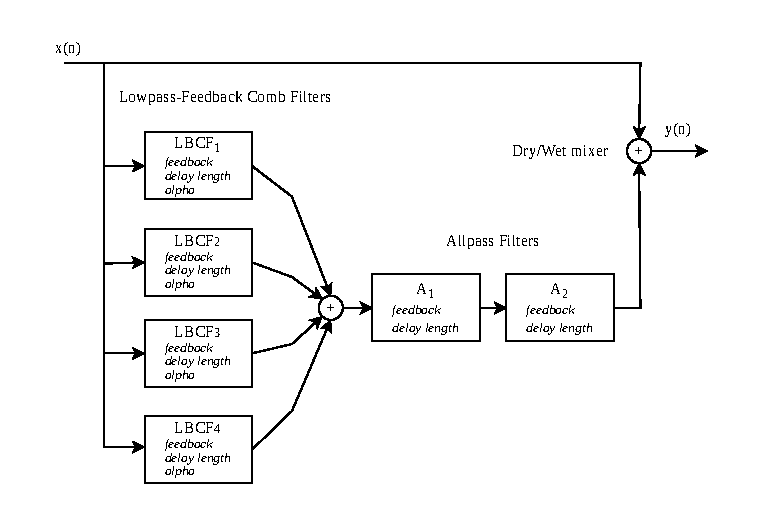
\includegraphics[width=0.8\textwidth]{../images/schroeder_reverb/schroeder_reverb.drawio.pdf}
	}
	\vspace{-2em}
	\caption{Schroeder Reverb Block Diagram}
	\label{fig:schroeder_block}
\end{figure}

Figure \ref{fig:schroeder_block} shows the basic structure of the implemented reverb.
Cursive parameters, such as filter coefficient \textit{alpha}, the \textit{feedback} gain and \textit{delay length}, are implemented as controllable by outside of the component.

The combination of parallel comb filters feeding into series allpass filters is a psychoacoustically motivated design. 
The comb filters produce the characteristic frequency-domain coloration and exponential decay of a reverberant space, but their echo density is too sparse on its own. 
The allpass filters, also called \textit{diffusers}, increase the echo density without adding frequency coloration, since their magnitude response is flat across all frequencies. 
Together, the structure achieves both a perceptually convincing decay envelope and a sufficiently dense late reverberation tail. \cite[p.~97]{juliuso.smithPhysicalSignalProcessing}

\subsubsection{Feedback Comb Filter}
\label{sec:comb_filter}

At the basis of the \textit{Schroeder Reverberator} is a structure of parallel comb filters.
Comb filters are fundamental building blocks for digital audio effects. 
Its most obvious example is a simple echo implementation \cite[p.~57]{juliuso.smithPhysicalSignalProcessing}.

The most simple variant is a \textit{feedforward} comb filter. It takes the input signal $x[n]$ and adds a delayed copy, shifted by $D$ samples, to produce the output $y[n]$. Since the delayed signal is not fed back into the input, each reflection occurs only once.

In theory, a room reverberation simulation can be constructed using only \textit{feedforward} 
comb filters, where each reflection is modelled by a separate filter instance. 
In practice however, this becomes computationally expensive for a convincing 
reverb with many reflections.~\cite[p.~85]{juliuso.smithPhysicalSignalProcessing}

\begin{figure}[H] \vspace{-1em} \centering \makebox[\textwidth][c]{ 			
	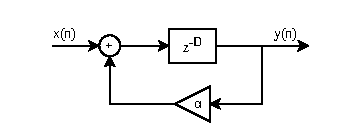
\includegraphics[width=0.5\textwidth]{../images/schroeder_reverb/comb.drawio.pdf}} 
	\vspace{-2em} 
	\caption{Feedback Comb Filter}  
	\label{fig:schroeder_comb} 
\end{figure}


Where the \textit{feedforward} comb filter implements an FIR filter, the \textit{feedback} comb filter (Figure \ref{fig:schroeder_comb}) takes the delayed output and feeds it back to the input. This filter type is also known as an IIR (Infinite Impulse Response) or \textit{recursive} filter, and is described by the difference equation:
\begin{equation}
y[n] = x[n] + \alpha \cdot y[n - D]
\end{equation}
where $\alpha$ is the feedback gain and $D$ the delay in samples.

The feedback comb filter can be understood as a physical model of a series of 
exponentially decaying echoes, resembling a signal reflecting between two parallel 
walls. For this reason, feedback comb filters are preferred in reverb design, 
offering a more natural decay while remaining computationally 
efficient. \cite[p.~98]{juliuso.smithPhysicalSignalProcessing}

\begin{wrapfigure}{r}{0.57\textwidth}
	\centering
	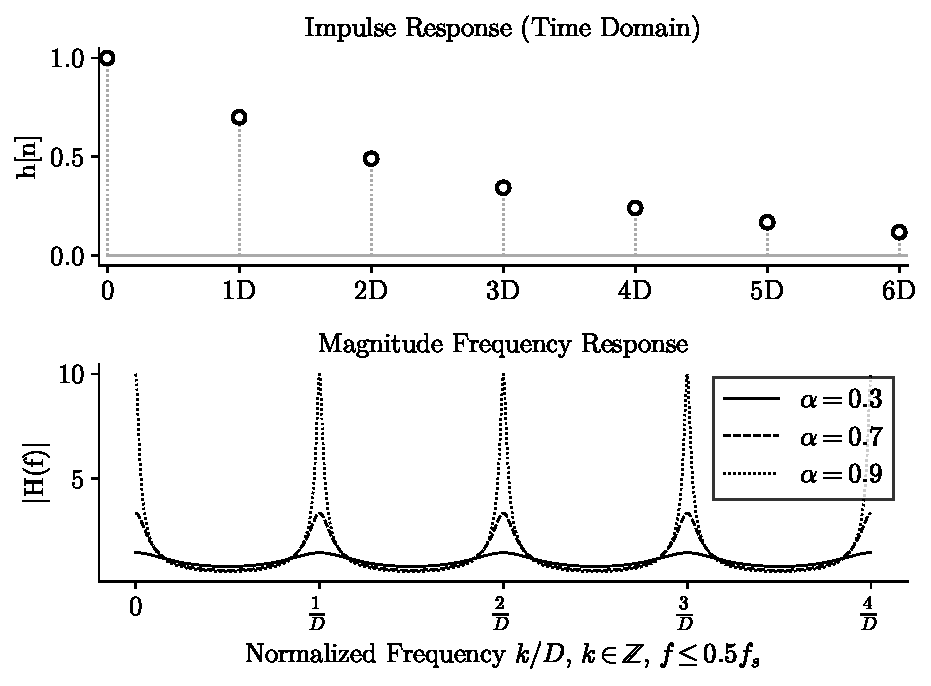
\includegraphics[width=0.54\textwidth]{../images/schroeder_reverb/fig_comb_filter_response.pdf}
	\caption{Impulse and Frequency Response of Feedback Comb Filter with different feedback gain $\alpha$}
	\label{fig:schroeder_comb_filter_response}
\end{wrapfigure}

The feedback coefficient $\alpha$ must be less than 1 in magnitude for the filter to be stable. 
Otherwise each echo would be louder than the previous one, causing the output to diverge and become unstable.

A feedback gain close to $1$ produces a very slowly decaying tail, which can be an interesting
artistic effect but must be used with caution. 

In Figure~\ref{fig:schroeder_comb_filter_response} the decaying echoes at uniform intervals of
$D$ samples are clearly visible in the impulse response.
The characteristic frequency response resembling a comb gives the filter its name.
The evenly spaced peaks arise because constructive interference occurs at every integer multiple
of $f_s/D$, producing resonances separated by $1/D$ in normalized frequency.

Essentially the peaks are frequencies where the delay $D$ is an exact multiple of the period of that frequency. 
The delayed copy arrives back perfectly in phase with 
the new input, and they reinforce each other. At the troughs, the input signal is exactly \textit{out of phase} with the fed-back delayed signal, causing cancellation.

\paragraph{Lowpass-Feedback Comb Filter}

Instead of using a standard feedback comb filter, this project employs a \textit{lowpass-feedback} comb filter (\ac{LBCF}), which places a filter $H_f(z)$ in the feedback path alongside the feedback gain $\alpha$.

\begin{figure}[H]
	\centering
	\vspace{-1.5em}
	\makebox[\textwidth][c]{%
		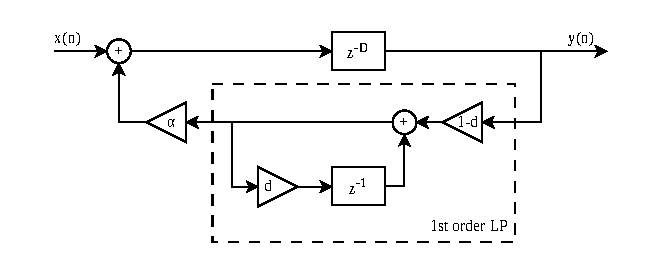
\includegraphics[width=0.7\textwidth]{../images/schroeder_reverb/lp_filtered_comb.drawio.pdf}
	}
	\vspace{-2.0em}
	\caption{Filtered-Feedback Comb Filter with 1st order Lowpass}
	\label{fig:schroeder_lbcf}
\end{figure}

The transfer function in the $z$-domain is given by:

\begin{equation}
	H_{LBCF}(z) = \frac{z^{-D}}{1 - \alpha \cdot H_{f}(z) \cdot  z^{-D}}
\end{equation}

Note that the transfer function is given here with the output taken after the delay, differing slightly from the notation in \cite{juliuso.smithPhysicalSignalProcessing}.
 
Using a first-order lowpass $H_f(z) = H_{lp}(z)$ with a damping coefficient $d$:
\begin{equation}
	H_{lp}(z) = \frac{1 - d}{1 - d \cdot z^{-1}}
\end{equation}

the full transfer function becomes:

\begin{equation}
H_{LBCF}(z) = \frac{z^{-D}}{1 - \alpha \frac{1 - d}{1 - d \cdot z^{-1}}  z^{-D}}
\end{equation}

The effect of the lowpass in the feedback path causes high frequencies to decay faster than low frequencies, producing a more natural reverb tail. 
Adding a low-pass filter in the feedback loop can effectively recreate the losses that happen when a signal travels back and forth between two places, as happens in real rooms. \cite[p.~62]{juliuso.smithPhysicalSignalProcessing}


\begin{wrapfigure}{r}{0.57\textwidth}
	\centering
	\vspace{-2.0em}
	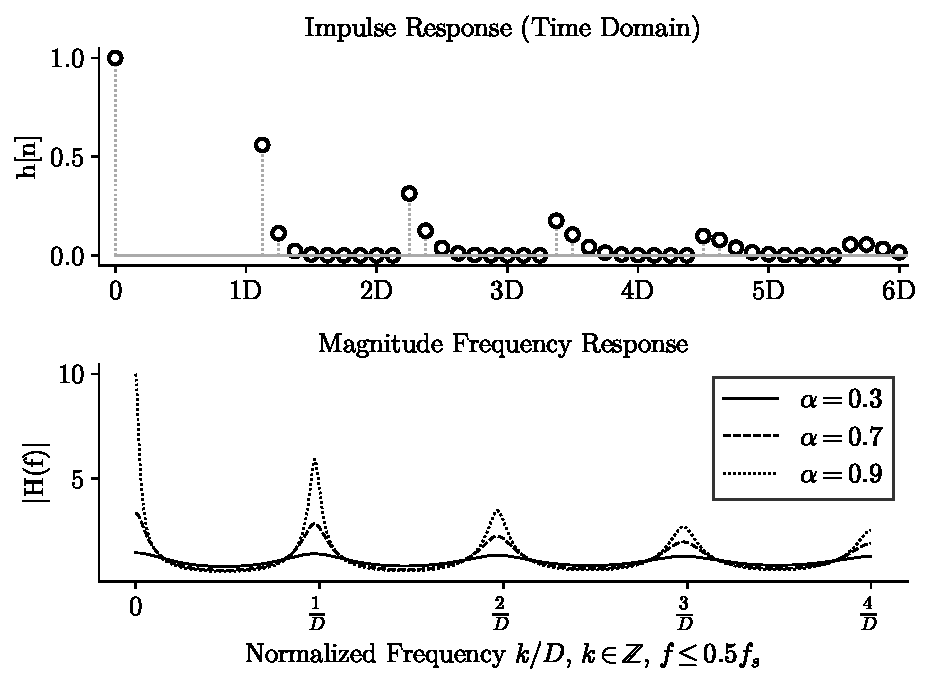
\includegraphics[width=0.55\textwidth]{../images/schroeder_reverb/fig_comb_filter_lp_feedback_response.pdf}
	\caption{Impulse and Frequency Response of Lowpass Feedback Comb Filter with different feedback gain $\alpha$ and filter coefficient $d=0.2$}
	\label{fig:schroeder_comb_filter_lp_feedback_response}
\end{wrapfigure}

\paragraph{Impulse and Frequency Response} 
In Figure~\ref{fig:schroeder_comb_filter_lp_feedback_response}, the effect of the lowpass filter in the feedback path is clearly visible. 

Compared to the pure feedback comb filter in Figure \ref{fig:schroeder_comb_filter_response}, the impulse response shows non-zero samples between the echo peaks, caused by the smearing effect of the one-pole IIR filter.

In the frequency response, the comb peaks are attenuated at higher frequencies, as the lowpass reduces the feedback gain progressively with frequency, resulting in shorter decay times for high frequencies than for low frequencies.

\clearpage
\subsubsection{Allpass Filter}

The allpass filter passes all frequencies at equal gain. 
Unlike lowpass or highpass filters, it does not attenuate any frequency band. 
Instead, it affects only the \textit{phase} of the signal, introducing frequency-dependent delays while leaving the magnitude response flat at unity gain across all frequencies. 
In the context of the Schroeder reverberator, allpass filters are used as \textit{diffusers}: they increase the echo density of the late reverberation without coloring the sound, complementing the tonal decay provided by the comb filter bank. \cite{juliuso.smithPhysicalSignalProcessing}

\begin{figure}[H]
	\centering
	\makebox[\textwidth][c]{%
		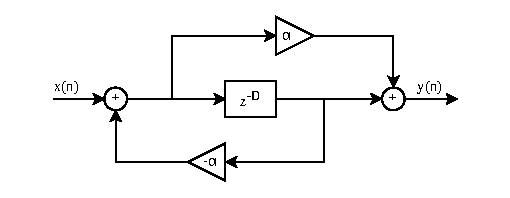
\includegraphics[width=0.6\textwidth]{../images/schroeder_reverb/allpass.drawio.pdf}
	}
	\caption{Allpass Filter}
	\label{fig:schroeder_allpass}
\end{figure}

The allpass filter can be constructed by cascading a \textit{feedforward} and \textit{feedback} comb filter delay line (see Section \ref{sec:comb_filter}). Figure \ref{fig:schroeder_allpass} illustrates the combination of the two comb filter variants. \cite[p.69]{juliuso.smithPhysicalSignalProcessing}
 \\

When inspecting the transfer function:
\begin{equation}
	H(z) = \frac{\alpha + z^{-D}}{1 + \alpha z^{-D}}
\end{equation}

It becomes clear, how the Schroeder allpass works. The numerator and denominator of $H(z)$ are mirror images of each other. 

\vspace{2.0em}

\begin{wrapfigure}{r}{0.57\textwidth}
	\centering
	\vspace{-2.0em}
	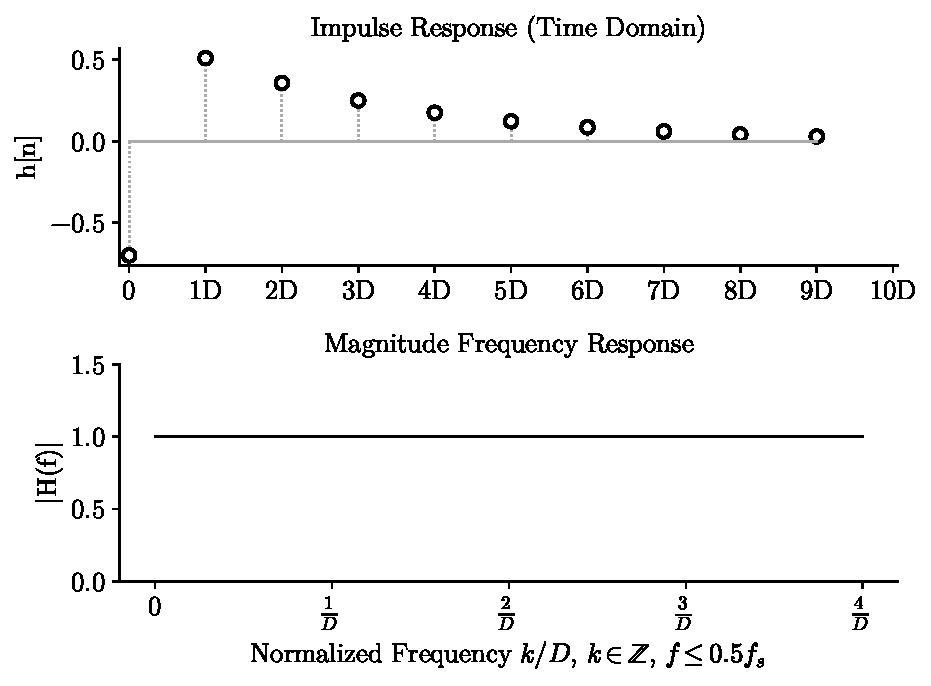
\includegraphics[width=0.55\textwidth]{../images/schroeder_reverb/fig_allpass_response.pdf}
	\caption{Impulse and Frequency Response of Allpass Filter}
	\label{fig:schroeder_allpass_filter_response}
\end{wrapfigure}


Whatever the feedback amplifies at a certain frequency, the feedforward cancels exactly, leaving only a phase shift (the delay in time-domain) behind.  
This causes the totally flat frequency response of the \textit{allpass} filter.
Note the similar impulse response to the feedback comb filter \ref{fig:schroeder_comb_filter_response}

\clearpage
\subsection{Design and Implementation}
% 4-comb + 2-allpass, LP damping in comb feedback path, prime stereo decorrelation.

The implemented reverberator follows a simplified variant of the \textit{Freeverb} \cite{freeverb-github} variant of the Schroeder structure -- a public-domain C++ program, used extensively in the free-software community -- adapted here for embedded C on a microcontroller target. 

It consists of four parallel lowpass-feedback comb filters summing into two series allpass filters, per channel \cite[p.~101]{juliuso.smithPhysicalSignalProcessing}. The full z-domain block diagram is shown in Figure~\ref{fig:schroeder_block_detailed}.

\begin{figure}[htbp]
	\centering
	\vspace{-1.1em}
	\makebox[\textwidth][c]{
		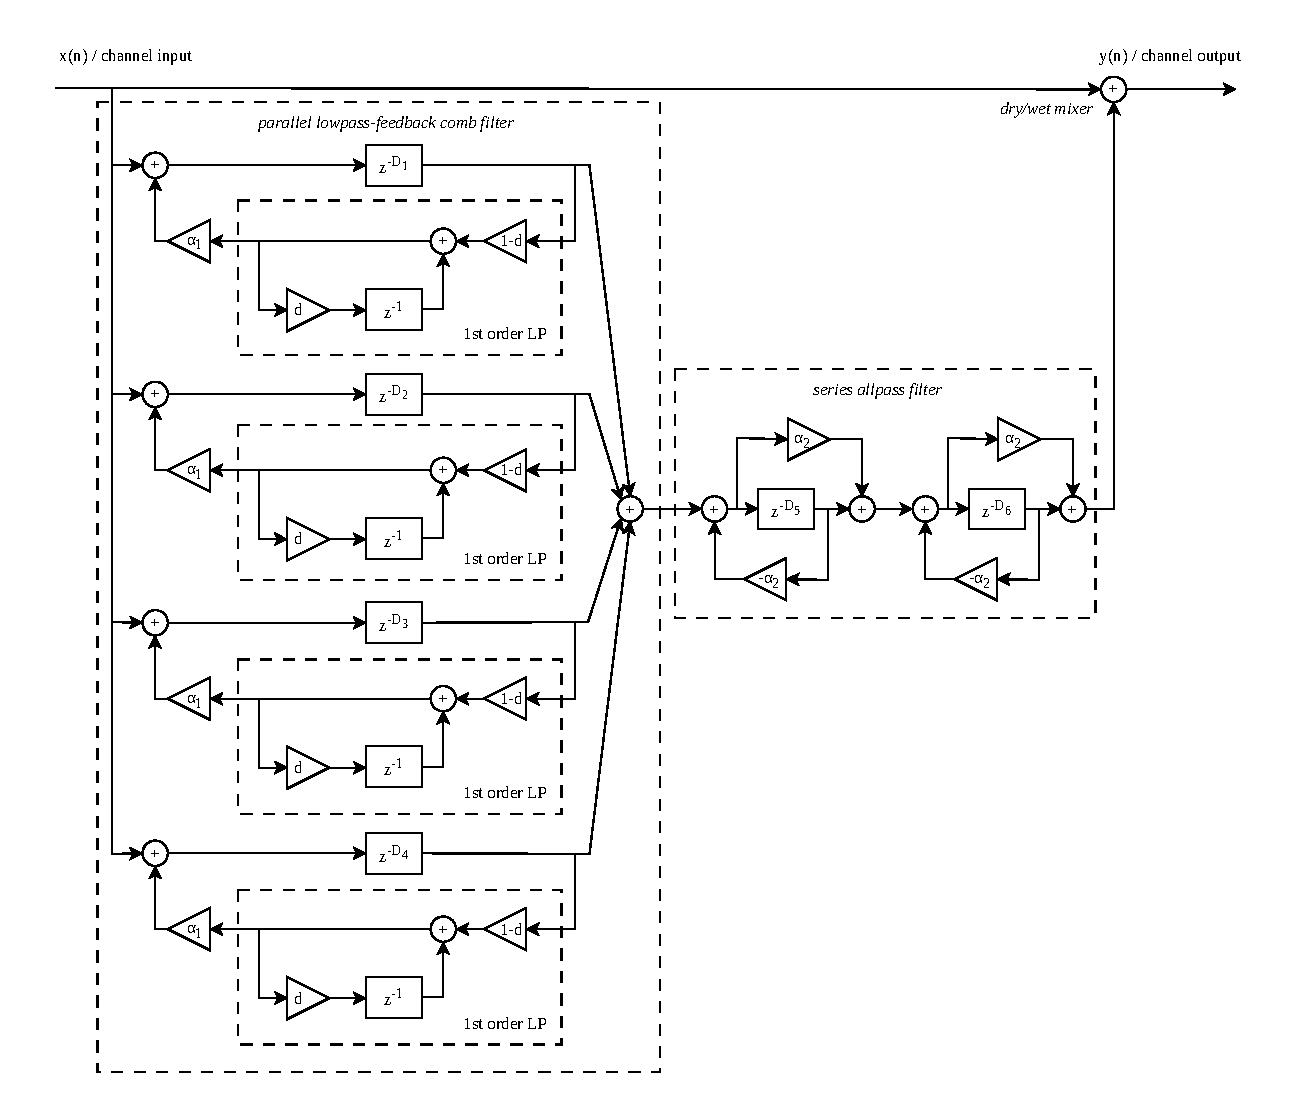
\includegraphics[width=1.1\textwidth]{../images/schroeder_reverb/schroeder_reverb_block_detailed.drawio.pdf}	
		}
	\vspace{-2.0em}
	\caption{Schroeder Reverb Block Diagram}
	\label{fig:schroeder_block_detailed}
\end{figure}

\vspace{-2.0em}

\paragraph{Delay Line Structure} Each filter (comb or allpass) is backed by a statically allocated circular float buffer that holds the sample history required by the delay line. 
Both filters share the same \texttt{sr\_delay\_t} struct, which stores the buffer pointer, its maximum allocated \texttt{size}, the currently active \texttt{length}, and a write index \texttt{idx}. 
Separating \texttt{size} from \texttt{length} allows the active delay time to be changed at runtime without reallocating memory. 
The struct also carries filter-specific state: \texttt{feedback} gain and \texttt{lp\_state} for the comb filter's damped feedback path.

\begin{listing}[H]
\begin{minted}{c}
typedef struct {
	float feedback;
	float* buf;
	uint32_t size;   /**< Buffer capacity in samples. */
	uint32_t idx;
	uint16_t length; /**< Active delay length in samples (<= size). */
	
	float lp_state;
	float lp_alpha;  /**< One-pole LP coefficient in the comb feedback path. */
} sr_delay_t;
\end{minted}
\vspace{-2.0em}
\caption{delay-line struct type definition}
\label{lst:schroeder-delayline-struct}
\end{listing}

\vspace{-2.5mm}	
The functionality of both, the comb- and allpass filters are implemented in the respective \texttt{*\_process} functions:

\begin{listing}[H]
\vspace{-2.5mm}	
\begin{minted}[linenos]{c}
static float comb_process(sr_delay_t* d, float in) {
	// calculate read index with wraparound depending on set .length parameter
	uint32_t read_idx = (d->idx + d->size - d->length) % d->size;
	float y = d->buf[read_idx];
	
	float feedback_signal = y * d->feedback;
	
	// one-pole lowpass on each combs fb path.
	d->lp_state = (1.0f - d->lp_alpha) * feedback_signal + d->lp_alpha * d->lp_state;
	d->buf[d->idx] = in + d->lp_state;
	
	d->idx++;
	if (d->idx >= d->size)
	d->idx = 0;
	
	return y;
}

static float allpass_process(sr_delay_t* d, float in) {
	// calculate read index with wraparound depending on set .length parameter
	uint32_t read_idx = (d->idx + d->size - d->length) % d->size;
	float buf = d->buf[read_idx];
	
	float y = -in + buf;
	d->buf[d->idx] = in + buf * d->feedback;
	
	d->idx++;
	if (d->idx >= d->size)
	d->idx = 0;
	
	return y;
}
\end{minted}
\vspace{-2.0em}
\caption{process functions of comb and allpass filters}
\label{lst:schroeder-process-functions}
\end{listing}


Both underlying \texttt{sr\_delay\_t} structures share the same ring buffer mechanics: \texttt{idx} advances by one each tick, and the delay tap is read from \mintinline{c}|(idx + size - length) % size|, placing it exactly \texttt{length} samples behind the write head in O(1) without branching.

The comb filter runs the feedback sample through a one-pole lowpass (line 9) before writing it back with the input (line 10), implementing damped feedback in-place. 
The allpass uses the same ring structure but applies the Schroeder topology (lines 22--25) directly, yielding flat magnitude response with phase dispersion.

\paragraph{Static Memory Allocation} 
\label{sec:schroeder_memory_allocation}

Twelve buffers are allocated in total: eight comb buffers of \texttt{MAX\_COMB\_LEN}~=~1620 samples and four allpass buffers of \texttt{MAX\_AP\_LEN} = 600 samples. At 32-bit float precision (4 bytes per sample), the total static memory footprint is:
\begin{equation}
(8 \times 1620 + 4 \times 600) \times 4\ \text{bytes} = 61.4\ \text{kB}
\end{equation}

The buffer size and thus the maximum delay lengths are directly correlated to the maximum room size of the algorithm. 
Increasing the base delay lengths would produce a larger perceived space at \texttt{size = 1}, at the cost of higher memory consumption. 
%The current values were chosen to provide an aesthetically pleasing maximum room size while maintaining a conservative memory footprint, preserving available RAM for the sample playback buffers in the system.

\paragraph{Delay Length Selection} Using mutually prime delay line lengths, i.e. values sharing no common factors, helps avoid spectral clustering and unnatural resonances in the frequency response. 
When delay lengths share common factors, their resonant frequencies align, causing certain frequencies to be disproportionately reinforced. By choosing mutually prime lengths, the resonances are maximally spread across the spectrum, resulting in a evenly decay envelope.
The delay lengths were selected empirically by ear from prime numbers, starting from a base set and scaled by a room size parameter. 
The comb delays (30--34\,ms) target the late reverberation tail, while the allpass delays are kept short (5--12\,ms) to increase echo density without introducing perceivable discrete echoes. 
The chosen base delay lengths are:

\begin{table}[H]
    \centering
    \begin{tabular}{lcccc}
        \hline
        & \multicolumn{4}{c}{Comb Filter Delays (samples)} \\
        & 1 & 2 & 3 & 4 \\
        \hline
        Left  & 1553 & 1613 & 1499 & 1427 \\
        Right & 1567 & 1601 & 1487 & 1433 \\
        \hline
    \end{tabular}
    \hspace{2em}
    \begin{tabular}{lcc}
        \hline
        & \multicolumn{2}{c}{Allpass Delays (samples)} \\
        & 1 & 2 \\
        \hline
        Left  & 223 & 557 \\
        Right & 229 & 563 \\
        \hline
    \end{tabular}
    \caption{Base delay line lengths for comb and allpass filters (in samples at \qty{48}{\kilo\hertz}).}
    \label{tab:delay-lengths}
\end{table}

The slight asymmetry between left and right channels provides stereo decorrelation, widening the perceived sound field without additional processing.

\paragraph{Stability and Feedback Scaling} To prevent instability as the room size parameter is reduced, the feedback gain is scaled automatically using two macros:

\begin{verbatim}
	#define COMB_FEEDBACK(size)   (0.97f + 0.01f * (1.0f - size))
	#define ALLPASS_FEEDBACK(size)(0.68f + 0.01f * (1.0f - size))
\end{verbatim}

As the room size decreases, delay lines shorten and the filter accumulates energy more rapidly. 
The macros compensate by slightly increasing the base feedback value as size decreases, maintaining a perceptually consistent decay across the full parameter range. 
The feedback value passed in by the user is additionally clamped to $[0,0.999]$ before being applied, ensuring the filter never reaches the instability threshold of $\alpha = 1$. 
A minimum room size of 0.30 is enforced to prevent the delay lines from becoming so short that the filter becomes difficult to stabilise.

\paragraph{Controllable Parameters}
\begin{center}
    \small
    \begin{tabular}{ll}
        \toprule
        \textbf{Parameter} & \textbf{Description} \\
        \midrule
        \texttt{wet}            & Dry/wet balance; $\texttt{dry} = 1 - \texttt{wet}$ enforced automatically. \\
        \texttt{feedback} $(\alpha)$ & RT60 decay time; routed through stability macros to compensate for room size. \\
        \texttt{size}           & Uniformly scales all delay lengths, preserving prime relationships. \\
        \texttt{lp\_alpha} $(d)$  & One-pole IIR cutoff in each comb path; attenuates highs for natural decay. \\
        \bottomrule
    \end{tabular}
\end{center}

\paragraph{Parameter Coupling}
\label{sec:schroeder_parameter_coupling}
The feedback gain and room size parameters are implicitly coupled through the stability macros. The \texttt{size} scalar is stored in the \texttt{schroeder\_stereo\_t} struct so that \\ \texttt{schroeder\_rev\_set\_feedback} can reference it when computing the scaled feedback values:
\begin{minted}{c}
	float comb_fb = feedback * COMB_FEEDBACK(rev->size);
\end{minted}

\section{Verification and Testing}
\subsection{Hardware Testing}
\subsubsection{Power and safety tests}

\subsubsection{Signal integrity measurements}
\input{input_signal_test.tex}

\subsubsection{Noise and distortion measurements}

\subsection{Firmware Testing}
\subsubsection{Driver verification}

\subsubsection{Timing and latency analysis}

\subsubsection{Calibration accuracy}

\subsection{System-Level Validation}

End-to-end signal tests/loopback?

Eurorack compatibility tests

\section{Results and Evaluation}
\subsection{Measured performance vs requirements}

\subsection{Audio quality evaluation}

\subsection{Calibration accuracy and stability}

\subsubsection{Discussion of limitations}

\newpage
\addcontentsline{toc}{section}{References}
\printbibliography
	
\end{document}
